% Provenance (never printed): see sources/outline_sources.md (Year 3:
% ocean dynamics: the Ekman layer derived, the Sverdrup balance, western
% intensification, the abyssal circulation, ocean tides).
% Brief: sources/book5/BRIEFS.md, ch. 21. Curves from
% figdata/bachelor-3/wind_driven_gyre.py and tides.py. Exercise and problem
% values in the Book 5 scratch calculator calc/ch21.py. The basins, winds
% and stations of the exercises and the problem are invented.
\chapter{Dinâmica dos oceanos}\label{ch:b3:ocean-dynamics}

Pelo estreito da Flórida, a corrente do Golfo transporta cerca de
\qty{32}{\sverdrup} de água para o norte, e ela cresce à medida que acompanha a costa
para o norte, até cerca de \qty{150}{\sverdrup} perto de \ang{40} N. Do outro lado do mesmo oceano, ao largo de Portugal e do norte
da África, nada parecido flui para o sul: a água que a corrente do Golfo transporta
para o norte retorna em direção ao equador como uma deriva lenta e ampla, por milhares
de quilômetros de mar aberto. Toda bacia oceânica do Hemisfério Norte tem
o mesmo formato assimétrico, com a sua corrente rápida no lado oeste. A
assimetria decorre do vento, do atrito do mar e de um
fato sobre a Terra: o parâmetro de Coriolis cresce em direção ao polo.
% ledger: rapid:transports (31.7 Sv, rounded), stewart:north-atlantic

\begin{recall}
A força de maré da Lua e do Sol, as marés de sizígia e de quadratura, estão nos
volumes de física. A tensão do vento, a camada de Ekman, o transporte de Ekman e
a espiral de Ekman, a ressurgência e o afundamento, os giros, as correntes
de contorno oeste, o sverdrup ($\qty{1}{\sverdrup} =
\qty{e6}{m^3/s}$), a circulação meridional de revolvimento e a
formação de água profunda estão no volume do primeiro ano, no seu capítulo sobre a
circulação oceânica; ali a tensão do vento é escrita $\vec T$, aqui
$\vec\tau$. O parâmetro de Coriolis, o plano $\beta$, o raio de Rossby
e o equilíbrio geostrófico estão no Capítulo~\ref{ch:b3:gfd-foundations};
a vorticidade e a \omterm{def:b3:atmospheric-dynamics:pv}{vorticidade potencial} no Capítulo~\ref{ch:b3:atmospheric-dynamics}.
\end{recall}

\section{A camada de Ekman deduzida}\label{sec:b3:ocean-dynamics:ekman}

No volume do primeiro ano, o transporte de Ekman foi obtido a partir de um balanço de forças
sobre toda a camada, e a espiral de velocidades em seu interior foi enunciada. Com
um atrito de viscosidade turbulenta constante $A_z$, a espiral decorre
das equações em poucas linhas. Escreve-se a velocidade horizontal como um
número complexo, $W = u + \mathrm iv$, e a tensão do vento como $\tau =
\tau_x + \mathrm i\tau_y$; a multiplicação por $-\mathrm i$ faz girar um vetor
de \ang{90} no sentido horário, para a sua direita vista de cima.

\begin{theorem}[Perfil de velocidades de uma camada superficial estacionária forçada pelo vento]\label{thm:b3:ocean-dynamics:ekman}
Em um oceano estacionário, horizontalmente uniforme, de grande profundidade e densidade constante
$\rho$, com viscosidade turbulenta vertical constante $A_z$ e o
parâmetro de Coriolis $f > 0$, a corrente gerada por uma tensão do vento $\tau$ é
\[
W(z) = W_0\,\mathrm e^{(1+\mathrm i)z/\delta},\qquad
W_0 = \frac{\tau}{\rho\sqrt{fA_z}}\,\mathrm e^{-\mathrm i\pi/4},\qquad
\delta = \sqrt{\frac{2A_z}{f}} ,
\]
para $z \le 0$. A corrente superficial é girada de \ang{45} à direita da
tensão; com a profundidade ela gira ainda mais para a direita e decai como $\mathrm
e^{z/\delta}$; o transporte total $\int_{-\infty}^0 W\,\mathrm dz =
-\mathrm i\tau/(\rho f)$ é perpendicular à direita da tensão.
\end{theorem}

\begin{proof}
Longe das costas não há gradiente horizontal de pressão na camada,
e a força de Coriolis equilibra o atrito: $-fv = A_z u''$ e $fu =
A_z v''$, com os apóstrofos indicando derivadas em $z$. Multiplicando a segunda por
$\mathrm i$ e somando obtém-se $A_zW'' = \mathrm ifW$. Suas soluções são
$\mathrm e^{\pm(1+\mathrm i)z/\delta}$, pois $(1+\mathrm i)^2/\delta^2 =
2\mathrm i/\delta^2 = \mathrm if/A_z$; apenas o sinal de mais permanece limitado quando
$z \to -\infty$. Na superfície, a tensão é transmitida pelo atrito,
$\rho A_zW'(0) = \tau$, logo $W_0 = \tau\delta/(\rho A_z(1+\mathrm i))$.
Como $\delta/(\sqrt2 A_z) = 1/\sqrt{fA_z}$ e $1/(1+\mathrm i) = \mathrm
e^{-\mathrm i\pi/4}/\sqrt2$, isso é o $W_0$ enunciado. O fator
$\mathrm e^{\mathrm iz/\delta}$ gira no sentido horário quando $z$ diminui. Por fim
$\int_{-\infty}^0 W\,\mathrm dz = W_0\delta/(1+\mathrm i) =
\tau\delta^2/(\rho A_z(1+\mathrm i)^2) = \tau\delta^2/(2\mathrm i\rho A_z)
= -\mathrm i\tau/(\rho f)$.
\end{proof}

O teorema recupera os dois resultados do volume do primeiro ano: a corrente
superficial de Ekman, girada de \ang{45}, e o transporte $\tau/(\rho f)$, perpendicular à
tensão e independente de $A_z$, grandeza que nunca é bem conhecida. Na
profundidade $\pi\delta$, a corrente flui em sentido oposto à corrente superficial, reduzida
por $\mathrm e^{-\pi}$, para \qty{4}{\percent}.

\begin{definition}[Profundidade de Ekman; bombeamento de Ekman]\label{def:b3:ocean-dynamics:ekman-pumping}
A \emph{profundidade de Ekman}\index{profundidade de Ekman} é $D_E = \pi\delta =
\pi\sqrt{2A_z/f}$, a profundidade em que a corrente da espiral de Ekman
flui em sentido oposto à corrente superficial; ela mede a espessura da
camada de Ekman. O \emph{bombeamento de Ekman}\index{bombeamento de Ekman} é a
velocidade vertical $w_E$ na base da camada de Ekman, forçada pela convergência ou
divergência do transporte de Ekman: para baixo onde os transportes
convergem, para cima, chamada às vezes de sucção de Ekman, onde divergem.
\end{definition}

\begin{proposition}[Bombeamento de Ekman]\label{prop:b3:ocean-dynamics:pumping}
Com a velocidade vertical nula na superfície do mar, o \omterm{def:b3:ocean-dynamics:ekman-pumping}{bombeamento de Ekman} é
\[
w_E = \operatorname{curl}_z\frac{\vec\tau}{\rho f}
= \frac{1}{\rho f}\Big(\frac{\partial\tau_y}{\partial x} -
\frac{\partial\tau_x}{\partial y}\Big) + \frac{\beta\tau_x}{\rho f^2} ,
\]
com o sentido positivo para cima.
\end{proposition}

\begin{proof}
O transporte volumétrico da camada é $(U_E, V_E) = (\tau_y,
-\tau_x)/(\rho f)$, o teorema escrito em componentes. Integrando a
equação da continuidade $\partial w/\partial z = -(\partial u/\partial x +
\partial v/\partial y)$ através da camada, $w(0) - w_E = -(\partial
U_E/\partial x + \partial V_E/\partial y)$, logo $w_E = \partial_x(\tau_y/\rho
f) - \partial_y(\tau_x/\rho f)$. Expandindo com $\mathrm df/\mathrm dy =
\beta$ resulta na segunda forma.
\end{proof}

Um vento que gira ciclonicamente sobre o mar, com rotacional positivo, puxa
a água de baixo da camada para cima; um vento anticiclônico a empurra para baixo. Sobre
os oceanos subtropicais, os alísios sopram de leste no
lado equatorial, e os ventos de oeste no lado polar. Seus transportes de Ekman,
para norte sob os alísios e para sul sob os ventos de oeste,
convergem entre eles: a água superficial se acumula e é bombeada para baixo, como
na figura abaixo. Ao longo de uma costa onde o
vento sopra com a costa à sua esquerda (no Hemisfério Norte), o
transporte se afasta da margem, e a ressurgência costeira, tratada no
volume do primeiro ano, é uma sucção de Ekman concentrada contra uma parede.

\begin{omfigure}
\centering
\begin{tikzpicture}[>=stealth, font=\small, x=1.1cm, y=1cm]
\fill[omThm!7] (-5,0) rectangle (5,-3.6);
\draw[thick] (-5,0) -- (5,0);
\draw[black!45, densely dashed] (-5,-0.9) -- (5,-0.9);
\node[font=\scriptsize, black!60, anchor=north east, inner sep=1pt] at (4.95,-0.95) {camada de Ekman};
% winds: west is out of the page, east into the page
\foreach \x in {-4.2,-3.4,-2.6} {\draw (\x,0.55) circle (0.13); \fill (\x,0.55) circle (0.04);}
\foreach \x in {2.6,3.4,4.2} {\draw (\x,0.55) circle (0.13);
  \draw (\x-0.09,0.46) -- (\x+0.09,0.64); \draw (\x-0.09,0.64) -- (\x+0.09,0.46);}
\node[above] at (-3.4,0.75) {alísios, de leste};
\node[above] at (3.4,0.75) {ventos de oeste};
% Ekman transports converge
\draw[->, omDef, very thick] (-4.5,-0.45) -- (-1.2,-0.45);
\draw[->, omDef, very thick] (4.5,-0.45) -- (1.2,-0.45);
\node[omDef, font=\scriptsize, fill=omThm!7, inner sep=1pt] at (-2.85,-0.72) {transporte de Ekman};
% pumping
\foreach \x in {-0.6,0,0.6} \draw[->, omThm, thick] (\x,-0.55) -- (\x,-1.55);
\node[omThm, font=\scriptsize, anchor=west] at (0.75,-1.25) {$w_E < 0$};
% squashed column and Sverdrup flow
\draw[thick, black!70] (-0.62,-1.75) rectangle (0.62,-3.1);
\node[font=\scriptsize, black!70, align=center] at (0,-2.42) {coluna\\comprimida};
\draw[->, omMeth, very thick] (-0.75,-2.42) -- (-3.2,-2.42);
\node[omMeth, font=\scriptsize, align=center, above] at (-2.6,-2.40) {escoamento de Sverdrup,\\em direção ao equador};
\draw[black!45, densely dashed] (-5,-3.3) -- (5,-3.3);
\node[font=\scriptsize, black!60, anchor=south east, inner sep=1pt] at (4.95,-3.28) {base do escoamento forçado pelo vento};
\node[below, font=\scriptsize] at (-5,-3.6) {sul};
\node[below, font=\scriptsize] at (5,-3.6) {norte};
\end{tikzpicture}

\par\smallskip{\small Seção norte--sul de um giro subtropical
do Hemisfério Norte, com o leste apontando para dentro da página. Os transportes de Ekman sob os
alísios e os ventos de oeste convergem, a água é bombeada para baixo, e as
colunas abaixo, comprimidas, deslocam-se em direção ao equador, onde $f$ é menor,
para conservar sua \omterm{def:b3:atmospheric-dynamics:pv}{vorticidade potencial}.}\label{fig:b3:ocean-dynamics:pumping}
\end{omfigure}

\section{O balanço de Sverdrup}\label{sec:b3:ocean-dynamics:sverdrup}

Abaixo da camada de Ekman, o oceano é geostrófico. Uma coluna de água que é
comprimida pelo \omterm{def:b3:ocean-dynamics:ekman-pumping}{bombeamento de Ekman} deve, para conservar sua \omterm{def:b3:atmospheric-dynamics:pv}{vorticidade potencial} $f/h$,
deslocar-se para onde $f$ é menor: em direção ao equador. Em 1947, H.~U.~Sverdrup
tornou o argumento quantitativo para toda a profundidade do escoamento forçado pelo vento.
% ledger: stewart:ekman-layer (Sverdrup 1947)

\begin{theorem}[balanço de Sverdrup]\label{thm:b3:ocean-dynamics:sverdrup}
Em um oceano estacionário no qual os termos não lineares e o atrito lateral
são desprezíveis, o interior é geostrófico abaixo da camada de Ekman, e a
velocidade vertical se anula em alguma profundidade $-H$, o transporte volumétrico total para norte
por unidade de largura do escoamento forçado pelo vento obedece ao \emph{balanço
de Sverdrup}\index{balanço de Sverdrup}
\[
\beta V = \frac{1}{\rho}\operatorname{curl}_z\vec\tau
= \frac{1}{\rho}\Big(\frac{\partial\tau_y}{\partial x} -
\frac{\partial\tau_x}{\partial y}\Big) .
\]
\end{theorem}

\begin{proof}
No interior geostrófico $fv_g = \rho^{-1}\partial p/\partial x$ e
$fu_g = -\rho^{-1}\partial p/\partial y$. Logo $\partial_x(fu_g) +
\partial_y(fv_g) = 0$, ou seja, $f(\partial_xu_g + \partial_yv_g) + \beta
v_g = 0$ e, pela continuidade, $\beta v_g = f\,\partial w/\partial z$.
Integrando de $-H$, onde $w = 0$, até a base da camada de Ekman,
onde $w = w_E$, obtém-se $\beta V_g = fw_E$. Pela
\cref{prop:b3:ocean-dynamics:pumping}, $fw_E = \rho^{-1}\operatorname{curl}_z
\vec\tau + \beta\tau_x/(\rho f)$. Somando o transporte de Ekman $V_E =
-\tau_x/(\rho f)$, multiplicado por $\beta$, cancela o último termo:
$\beta(V_g + V_E) = \rho^{-1}\operatorname{curl}_z\vec\tau$.
\end{proof}

O balanço é notável pelo que dispensa: nem a profundidade do
escoamento, nem sua estrutura vertical, nem a viscosidade de turbilhão, apenas o
rotacional do vento e $\beta$. Sverdrup o derivou das equações de
movimento integradas até uma profundidade de movimento nulo, e testou-o contra as
seções hidrográficas dos navios de pesquisa \emph{Carnegie} e
\emph{Bushnell} no Pacífico tropical oriental, entre \ang{34} N e
\ang{10} S, com a profundidade de movimento nulo em \qty{1000}{m}: os transportes
calculados a partir do vento coincidiram com os obtidos do campo de densidade, mesmo
onde as correntes corriam contra o vento. Trabalhos posteriores, com ventos melhores,
encontraram a melhor concordância com uma profundidade de movimento nulo próxima de \qty{500}{m}, e
medições da tensão média no Pacífico equatorial em 1999 encontraram o
escoamento ali em \omterm{thm:b3:ocean-dynamics:sverdrup}{balanço de Sverdrup}. Saber se o balanço vale em toda parte é
mais difícil de demonstrar do que de supor: quase toda teoria da circulação oceânica
parte dele.
% ledger: stewart:sverdrup

Considere-se a bacia fictícia do problema deste capítulo: entre \ang{20} e
\ang{50} N, com \qty{6000}{km} de largura, sob uma tensão zonal $\tau_x =
-\tau_0\cos(\pi(\varphi - \ang{20})/\ang{30})$ com $\tau_0 =
\qty{0.1}{Pa}$, de leste em \ang{20} N, de oeste em \ang{50} N, nula em
\ang{35} N. Sobre quase toda a bacia o rotacional da tensão é negativo: a
água é bombeada para baixo, cerca de \qty{35}{m} por ano em \ang{35} N, e o
interior escoa para o sul, \qty{4.9}{m^2/s} por metro de largura em \ang{35} N,
\qty{29.4}{\sverdrup} através da bacia. Calculado a partir dos ventos observados,
o transporte de Sverdrup do giro subtropical do Atlântico Norte atinge cerca de
\qty{30}{\sverdrup} próximo de \ang{28} N.
% ledger: stewart:north-atlantic (computed in figdata/bachelor-3/wind_driven_gyre.py)

\begin{omfigure}
\begin{tikzpicture}
\begin{groupplot}[group style={group size=3 by 1, horizontal sep=0.45cm, yticklabels at=edge left},
  width=0.37\linewidth, height=0.46\linewidth, ymin=20, ymax=50, ytick={20,25,30,35,40,45,50},
  tick label style={font=\scriptsize}, label style={font=\small}, title style={font=\small}]
\nextgroupplot[xlabel={$\tau_x$ (\unit{Pa})}, ylabel={latitude (\unit{\degree} N)},
  xmin=-0.12, xmax=0.12, xtick={-0.1,0,0.1}, title={tensão do vento},
  scaled x ticks=false, xticklabel style={/pgf/number format/fixed}]
% computed in figdata/bachelor-3/wind_driven_gyre.py
\addplot[black!50, thin] coordinates {(0,20) (0,50)};
\addplot[omThm, thick] table[x=tau, y=lat] {figdata/out/bachelor-3-wind_driven_gyre-merid.dat};
\nextgroupplot[xlabel={$w_E$ (\unit{m/yr})}, xmin=-45, xmax=12, xtick={-40,-20,0},
  title={bombeamento de Ekman}]
\addplot[black!50, thin] coordinates {(0,20) (0,50)};
\addplot[omDef, thick] table[x=wE, y=lat] {figdata/out/bachelor-3-wind_driven_gyre-merid.dat};
\nextgroupplot[xlabel={transporte (\unit{\sverdrup})}, xmin=-32, xmax=10, xtick={-30,-20,-10,0,10},
  title={Sverdrup}]
\addplot[black!50, thin] coordinates {(0,20) (0,50)};
\addplot[omMeth, thick] table[x=Vtot, y=lat] {figdata/out/bachelor-3-wind_driven_gyre-merid.dat};
\end{groupplot}
\end{tikzpicture}

\par\smallskip{\small A bacia fictícia do problema, de \ang{20} a
\ang{50} N e com \qty{6000}{km} de largura. À esquerda, a tensão zonal do vento, positiva
para leste. No centro, o \omterm{def:b3:ocean-dynamics:ekman-pumping}{bombeamento de Ekman}, positivo para cima: a água é empurrada
para baixo ao sul de \ang{47} N, com mais intensidade no sul, onde $f$ é pequeno,
e puxada para cima ao norte dessa latitude. À direita, o transporte de Sverdrup total para o norte através da bacia:
o interior escoa para o sul, \qty{29.4}{\sverdrup} em \ang{35} N, exceto em uma
faixa estreita na borda norte, onde o rotacional da tensão muda de sinal.}\label{fig:b3:ocean-dynamics:sverdrup}
\end{omfigure}
% ledger: earth:Rmean, geod5:grs80-defining

O transporte de Sverdrup fixa $V$ em cada ponto, mas uma função de corrente
precisa de uma condição de contorno, e uma parede meridional só pode receber uma. Se o
interior não admite escoamento pela parede oriental, o escoamento para o sul
não tem para onde ir na parede ocidental; a massa retorna por uma corrente
que as equações de Sverdrup, sem atrito, não conseguem descrever.

\section{Intensificação ocidental}\label{sec:b3:ocean-dynamics:western}

Em 1948, H.~Stommel acrescentou o atrito mais simples ao oceano mais simples, e
encontrou o escoamento de retorno comprimido contra a parede ocidental, como na
figura do giro dele no volume do primeiro ano. Ele só obteve esse resultado com um parâmetro de Coriolis
que cresce para o norte: sem rotação, ou com um parâmetro uniforme,
o giro dele era simétrico.
% ledger: stewart:stommel, stommel:1948

\begin{definition}[Intensificação ocidental; modelo de Stommel; camada limite de Munk]\label{def:b3:ocean-dynamics:western-intensification}
A \emph{intensificação ocidental}\index{intensificação ocidental} é a
compressão do escoamento de retorno de um giro dirigido pelo vento em uma corrente estreita e
rápida contra o lado ocidental da bacia. O \emph{modelo de Stommel
}\index{modelo de Stommel} é um oceano homogêneo de profundidade constante em uma
bacia retangular, dirigido por uma tensão zonal do vento e freado por um atrito no fundo
proporcional à velocidade integrada na profundidade, com taxa $r$;
sua função de corrente de transporte $\psi$ ($U = -\partial\psi/\partial y$, $V =
\partial\psi/\partial x$) obedece a
\[
r\nabla^2\psi + \beta\frac{\partial\psi}{\partial x} =
\frac{1}{\rho}\operatorname{curl}_z\vec\tau ,\qquad \psi = 0 \text{ nas paredes.}
\]
A \emph{camada limite de Munk}\index{camada limite de Munk} é a
camada limite ocidental do mesmo giro quando uma viscosidade turbulenta lateral $A_H$
substitui o atrito no fundo; sua escala de largura é $\delta_M =
(A_H/\beta)^{1/3}$.
\end{definition}

A equação é o \omterm{thm:b3:ocean-dynamics:sverdrup}{balanço de Sverdrup} com o rotacional do atrito no fundo
acrescentado: integrada na profundidade, $\beta V = \rho^{-1}\operatorname{curl}_z
\vec\tau - r\zeta_T$, em que $\zeta_T = \nabla^2\psi$ é a vorticidade do
transporte.

\begin{theorem}[Camada limite ocidental do giro de Stommel]\label{thm:b3:ocean-dynamics:stommel}
Em uma bacia $0 \le x \le X$, $0 \le y \le L$, com $\tau_x = -\tau_0
\cos(\pi y/L)$ e $\delta_S = r/\beta \ll X$, a função de corrente de Stommel
é, até a ordem principal em $\delta_S/X$,
\[
\psi = A\sin\frac{\pi y}{L}\Big[(X - x) - X\mathrm e^{-x/\delta_S}\Big],
\qquad A = \frac{\pi\tau_0}{\rho\beta L} .
\]
O interior transporta $AX\sin(\pi y/L)$ para o sul; uma camada limite de largura
$\delta_S$ junto à parede ocidental o devolve para o norte; não pode existir
camada limite junto à parede oriental.
\end{theorem}

\begin{proof}
O rotacional da tensão é $-\partial\tau_x/\partial y = -(\pi\tau_0/L)\sin(\pi
y/L)$. Ao longo da largura da bacia, o termo de atrito é menor que o termo
$\beta$ por $\delta_S/X$; desprezando-o, resta o \omterm{thm:b3:ocean-dynamics:sverdrup}{balanço de Sverdrup},
$\beta\,\partial\psi/\partial x = -(\pi\tau_0/\rho L)\sin(\pi y/L)$, cuja
solução que se anula em $x = X$ é $\psi_I = A\sin(\pi y/L)(X - x)$. Ela não
se anula em $x = 0$. Junto a uma parede, $\psi$ varia rapidamente em $x$, e a
equação se reduz a $r\,\partial^2\psi/\partial x^2 + \beta\,\partial\psi/
\partial x = 0$ para a correção, cujas soluções são uma constante e
$\mathrm e^{-x/\delta_S}$. Esta última decai para leste, afastando-se da
parede ocidental: somando $-AX\sin(\pi y/L)\,\mathrm e^{-x/\delta_S}$, obtém-se $\psi = 0$
em $x = 0$ e nada muda no interior. Na parede oriental, uma
correção teria de decair para oeste, afastando-se de $x = X$, e
$\mathrm e^{-x/\delta_S}$ cresce para oeste: não há tal camada, de modo que o
interior precisa encontrar a parede oriental por si só, como faz $\psi_I$. O
transporte para o norte entre a parede e o ponto em que $V$ muda de sinal
é $\psi$ ali, próximo de $AX\sin(\pi y/L)$.
\end{proof}

A mesma resposta vem da vorticidade. Sobre o interior, o vento dá a
cada coluna vorticidade negativa, e a coluna a paga movendo-se
para o sul, em direção a valores menores de $f$. Na volta para o norte, ela ganha \omterm{def:b3:atmospheric-dynamics:vorticity-kinds}{vorticidade planetária}
e precisa perdê-la, o que só o atrito pode fazer. Em uma corrente para o norte
cuja velocidade cai para leste a partir de perto da parede ocidental, $\partial
v/\partial x < 0$ na maior parte de sua largura: a vorticidade da corrente é negativa, e o atrito, agindo contra
ela fornece a vorticidade positiva de que as colunas precisam. Uma corrente para o norte
junto a uma parede oriental teria vorticidade positiva, e
o atrito retiraria o sinal errado.

\begin{omfigure}
\begin{tikzpicture}
\begin{groupplot}[group style={group size=2 by 1, horizontal sep=1.7cm},
  width=0.48\linewidth, height=0.42\linewidth, xmin=0, xmax=400,
  xlabel={distância da parede ocidental (\unit{km})},
  tick label style={font=\scriptsize}, label style={font=\small},
  legend style={font=\scriptsize, draw=none, fill=none}]
\nextgroupplot[ylabel={$V$ (\unit{m^2/s})}, ymin=-80, ymax=600, legend pos=north east,
  legend cell align=left]
% computed in figdata/bachelor-3/wind_driven_gyre.py
\addplot[omThm, thick] table[x=x, y=vS] {figdata/out/bachelor-3-wind_driven_gyre-bl.dat};
\addlegendentry{Stommel, $\delta_S = \qty{53}{km}$}
\addplot[omDef, thick] table[x=x, y=vM] {figdata/out/bachelor-3-wind_driven_gyre-bl.dat};
\addlegendentry{Munk, $\delta_M = \qty{64}{km}$}
\addplot[black!50, thin, forget plot] coordinates {(0,0) (400,0)};
\nextgroupplot[ylabel={transporte a partir da parede (\unit{\sverdrup})}, ymin=0, ymax=36,
  legend pos=south east, legend cell align=left]
\addplot[omThm, thick] table[x=x, y=cS] {figdata/out/bachelor-3-wind_driven_gyre-bl.dat};
\addlegendentry{Stommel}
\addplot[omDef, thick] table[x=x, y=cM] {figdata/out/bachelor-3-wind_driven_gyre-bl.dat};
\addlegendentry{Munk}
\addplot[black!60, densely dashed] coordinates {(0,29.4) (400,29.4)};
\addlegendentry{interior, \qty{29.4}{\sverdrup}}
\end{groupplot}
\end{tikzpicture}

\par\smallskip{\small A camada limite oeste no meio da
bacia fictícia do problema (\ang{35} N, \qty{6000}{km} de largura). À esquerda, o
transporte para o norte por unidade de largura: a camada de Stommel, com atrito de fundo
$r = \qty{e-6}{s^{-1}}$, decai exponencialmente a partir da parede; a de Munk, com
$A_H = \qty{5e3}{m^2/s}$ e sem deslizamento na parede, cresce a partir de zero, atinge o máximo
a cerca de \qty{80}{km} da parede e é seguida por uma fraca contracorrente para o sul.
À direita, o transporte entre a parede e cada distância, em comparação com
os \qty{29.4}{\sverdrup} que o interior transporta para o sul: a camada de Stommel
acumula \qty{27.9}{\sverdrup} antes de seu escoamento se voltar para o sul, o jato de Munk
\qty{33.0}{\sverdrup} antes de sua contracorrente.}\label{fig:b3:ocean-dynamics:boundary}
\end{omfigure}
% ledger: stewart:munk

Com $r = \qty{e-6}{s^{-1}}$ a \ang{35} N, $\delta_S = \qty{53}{km}$, e
o escoamento para o norte ocupa os primeiros \qty{250}{km} a partir da parede. Em 1950,
W.~H.~Munk substituiu o atrito de fundo por uma viscosidade turbulenta lateral $A_H$,
que atua sobre o cisalhamento dentro da corrente; a equação ganha um termo
$A_H\nabla^4\psi$, e, junto à parede oeste, a correção passa a ser
$\mathrm e^{-x/2\delta_M}$ multiplicada por uma oscilação, $\cos(\sqrt3x/2\delta_M)$
e $\sin(\sqrt3x/2\delta_M)$. Com $A_H = \qty{5e3}{m^2/s}$, o jato para o norte
tem cerca de \qty{225}{km} de largura (\qty{233}{km} na bacia da figura),
com uma fraca contracorrente além dele, uma forma próxima à da corrente do Golfo e
à de Kuroshio. Como na camada de Stommel, o transporte do jato não
depende do atrito, mas apenas do rotacional da tensão do vento, da largura da
bacia e de $\beta$. A partir dos ventos de sua época, Munk calculou
\qty{36}{\sverdrup} para a corrente do Golfo e \qty{39}{\sverdrup} para a
Kuroshio, cerca da metade dos transportes então medidos; com um coeficiente de arrasto melhor
e médias mais finas da tensão, encontrou-se \qty{32}{\sverdrup}
para a corrente do Golfo em 1978. Medida principalmente com um cabo submarino, a
corrente do Golfo no Estreito da Flórida tem transportado \qty{31.7}{\sverdrup} em
média desde 2004. A jusante, ela cresce para cerca de \qty{150}{\sverdrup} perto de
\ang{40} N, e, ao largo do Cabo Hatteras, uma forte recirculação, que a teoria linear
não contém, prejudica a concordância.
% ledger: stewart:munk, rapid:transports, stewart:north-atlantic

\section{A circulação abissal}\label{sec:b3:ocean-dynamics:abyssal}

O oceano profundo é alimentado a partir de poucos lugares. No volume do primeiro ano, a água
profunda se forma onde a água superficial é resfriada e adensada no extremo norte
do Atlântico e ao redor da Antártida, e se espalha pelas bacias como Água Profunda do
Atlântico Norte e Água de Fundo Antártica. Entre 1958 e 1960,
H.~Stommel, A.~B.~Arons e A.~J.~Faller perguntaram como ela se espalha, usando o
mesmo argumento de vorticidade de Sverdrup.

\begin{definition}[modelo de Stommel--Arons]\label{def:b3:ocean-dynamics:abyssal}
O \emph{modelo de Stommel--Arons}\index{modelo de Stommel--Arons} da circulação abissal
supõe que a água profunda é suprida por convecção em poucas
fontes de alta latitude, e que a água retorna à parte superior do oceano por uma
ressurgência lenta e uniforme $W_0$ através da base da termoclina, equilibrada pela
mistura descendente de calor, e que o escoamento interior é geostrófico e conserva a
\omterm{def:b3:atmospheric-dynamics:pv}{vorticidade potencial}. A circulação fecha-se por correntes profundas de contorno
oeste.
\end{definition}

\begin{proposition}[Escoamento interior em direção aos polos do abismo]\label{prop:b3:ocean-dynamics:abyssal}
No \omterm{def:b3:ocean-dynamics:abyssal}{modelo de Stommel--Arons}, sobre um fundo plano, o transporte integrado em profundidade
para o norte do interior abissal é
\[
V = \frac{f}{\beta}W_0 = a\tan\varphi\,W_0 ,
\]
em direção aos polos nos dois hemisférios quando $W_0 > 0$.
\end{proposition}

\begin{proof}
Na região interior geostrófica, $\beta v = f\,\partial w/\partial z$, como na
demonstração do equilíbrio de Sverdrup. Integrando desde o fundo plano, onde
$w = 0$, até o topo da camada abissal, onde $w = W_0$, obtém-se $\beta V =
fW_0$, e $f/\beta = 2\Omega\sin\varphi\,a/(2\Omega\cos\varphi) =
a\tan\varphi$. No Hemisfério Sul, $\tan\varphi < 0$: o escoamento é
para o sul, novamente em direção aos polos.
\end{proof}

O resultado é contraintuitivo: o interior abissal escoa em direção às
fontes, não para longe delas. Stommel e Arons construíram experimentos em tanques em rotação
para se convencerem. A água das fontes percorre
as paredes ocidentais, em correntes profundas de contorno oeste que alimentam o interior
ao longo do caminho. Em um setor do oceano entre o equador e o polo, com toda a fonte $S_0$
junto ao polo, a corrente de contorno oeste
transporta $2S_0\sin\varphi$ em direção ao equador, o dobro da fonte no polo
e nada no equador: o excedente sobre $S_0$ é água recirculando
a partir do interior. O modelo faz com que a circulação profunda seja movida pela mistura,
e não pelo afundamento: sem a ressurgência, a convecção apenas encheria o
abismo com uma poça estagnada de água fria. Seus tempos de trânsito vão de
poucos séculos perto das fontes a quase mil anos no Pacífico
Norte. No fundo real do oceano, as cristas dividem as bacias, e a mistura é
intensa sobre topografia acidentada, e o escoamento profundo é muito mais zonal do que o
do modelo. Sua previsão duradoura é a corrente profunda de contorno oeste: no
Atlântico Norte, ela retorna cerca de \qty{14}{\sverdrup} de água a
\qty{2}{\celsius} para o sul, enquanto a corrente do Golfo leva a
água quente para o norte.
% ledger: stewart:stommel-arons, stewart:deep-circulation, stewart:heat-conveyor

\begin{omfigure}
\centering
\begin{tikzpicture}[>=stealth, font=\small, scale=0.95]
\fill[omThm!7] (0,0) -- (7,0) -- (4.2,5) -- (2.8,5) -- cycle;
\draw[thick] (0,0) -- (2.8,5) -- (4.2,5) -- (7,0);
\draw[black!45, densely dashed] (0,0) -- (7,0);
\node[below, font=\scriptsize] at (3.5,0) {equador};
\node[above, font=\scriptsize] at (3.5,5) {em direção ao polo};
\fill[omThm] (3.05,4.6) circle (0.17);
\node[font=\scriptsize, anchor=west, inner sep=1pt] at (3.22,4.6) {$S_0$};
% western boundary current
\draw[->, omThm, very thick] (2.75,4.35) -- (0.35,0.25);
\node[omThm, font=\scriptsize, rotate=60.8, inner sep=1pt] at (0.85,2.45) {corrente profunda de contorno oeste};
% interior poleward flow
\foreach \x/\y in {2.6/0.7, 3.8/0.7, 5.0/0.7, 3.1/1.7, 4.3/1.7, 3.6/2.7, 4.6/2.7} {
  \draw[->, omMeth, thick] (\x,\y) -- ++(0.15,0.65);}
% upwelling dots
\foreach \x/\y in {2.2/1.25, 3.4/1.25, 4.6/1.25, 5.6/1.25, 2.7/2.2, 3.9/2.2, 5.0/2.2, 3.3/3.2, 4.3/3.2, 3.8/3.9} {
  \draw[omDef] (\x,\y) circle (0.09); \fill[omDef] (\x,\y) circle (0.03);}
\node[omMeth, font=\scriptsize, align=left, anchor=west] at (6.45,2.6) {fluxo interior\\em direção ao polo};
\node[omDef, font=\scriptsize, align=left, anchor=west] at (6.6,1.5) {ressurgência $W_0$};
\end{tikzpicture}

\par\smallskip{\small A circulação abissal de Stommel--Arons em um setor
do oceano do Hemisfério Norte, vista de cima. A água profunda afunda em
uma fonte $S_0$ próxima ao polo, percorre em direção ao equador em uma
corrente profunda de contorno oeste e vaza para um interior que flui
em direção ao polo, subindo lentamente através da termoclina em toda parte (os
pontos, ressurgência voltada para o leitor).}\label{fig:b3:ocean-dynamics:stommel-arons}
\end{omfigure}

O interior do modelo, como o de Sverdrup, é geostrófico, e as
correntes geostróficas do mar profundo são medidas do mesmo modo que
Sverdrup as mediu: a partir da densidade.

\begin{definition}[Método dinâmico]\label{def:b3:ocean-dynamics:dynamic-height}
O \emph{método dinâmico}\index{método dinâmico} calcula a corrente geostrófica
entre duas estações hidrográficas a partir da densidade medida em
ambas, em relação a um nível de pressão de referência em que a corrente é tomada
como nula ou conhecida. A distância \omterm{def:b3:gravity-geodesy:geopotential}{geopotencial} entre duas superfícies de pressão,
$\int\alpha\,\mathrm dp$ com $\alpha = 1/\rho$ o volume específico, é
dividida em uma parte padrão, igual nas duas estações, e na
\emph{anomalia \omterm{def:b3:gravity-geodesy:geopotential}{geopotencial}} $\Delta\Phi$; a corrente na superfície superior,
perpendicular à linha entre as estações $A$ e $B$, distantes $L$
uma da outra, é
\[
v = \frac{\Delta\Phi_B - \Delta\Phi_A}{fL} .
\]
\end{definition}

Por que não medir a pressão diretamente, como fazem os meteorologistas? Uma corrente geostrófica
de \qty{10}{cm/s} a \ang{30} exige um gradiente de pressão de
\qty{7.5e-3}{Pa/m}, \qty{750}{Pa} ao longo de \qty{100}{km}: o peso de
\qty{7.4}{cm} de água do mar. Nenhum medidor de pressão no fundo do mar pode ser
nivelado com tanta precisão. A densidade, calculada com precisão de algumas partes por milhão,
fornece, em vez disso, a inclinação de uma superfície de pressão em relação a outra. A
água mais leve e mais quente fica à direita da corrente, olhando no sentido do escoamento,
no Hemisfério Norte. Através da corrente do Golfo, as superfícies de densidade constante
mudam de profundidade em mais de um quilômetro ao longo de \qty{100}{km}.
% ledger: stewart:dynamic-method

\begin{method}[Corrente geostrófica a partir de duas estações]\label{met:b3:ocean-dynamics:dynamic}
\begin{enumerate}
\item Em cada estação, calcule a anomalia de volume específico $\delta =
  \alpha(S, T, p) - \alpha(35, 0, p)$ a partir da salinidade,
  da temperatura e da pressão medidas.
\item Integre-a desde a pressão de referência até cada pressão $p$:
  $\Delta\Phi(p) = \int_p^{p_{\text{ref}}}\delta\,\mathrm dp$.
\item Em cada pressão, $v(p) = (\Delta\Phi_B - \Delta\Phi_A)/(fL)$ é
  a corrente em relação ao nível de referência, positiva com a estação $B$
  à direita.
\item Acrescente a corrente no nível de referência, se ela for conhecida, a partir de um flutuador
  à deriva ali ou da inclinação da superfície do mar medida por satélite.
\end{enumerate}
\end{method}

\begin{inthefield}[Uma matriz de flutuadores]
\begin{minipage}[t]{0.52\linewidth}\vspace{0pt}
\begin{dated}{2024}
Quase quatro mil flutuadores Argo percorrem o oceano mundial. Lançado
pela lateral de um navio, um flutuador afunda até cerca de \qty{1000}{m} e deriva
ali por cerca de nove dias; depois afunda até \qty{2000}{m} e sobe até a superfície,
medindo condutividade, temperatura e pressão no trajeto,
e o ciclo recomeça aproximadamente a cada dez dias; os flutuadores Deep Argo perfilam até
\qty{6000}{m}. Em julho de 2024, a matriz coletou seu trigésimo milionésimo
perfil. A partir dos perfis, os oceanógrafos calculam as anomalias geopotenciais
do \omterm{def:b3:ocean-dynamics:dynamic-height}{método dinâmico} em cada flutuador, e o deslocamento do próprio flutuador
entre duas emersões fornece a corrente média na profundidade de estacionamento:
a velocidade de referência que Sverdrup precisou supor agora é medida.
\end{dated}
\end{minipage}\hfill
\begin{minipage}[t]{0.44\linewidth}\vspace{0pt}
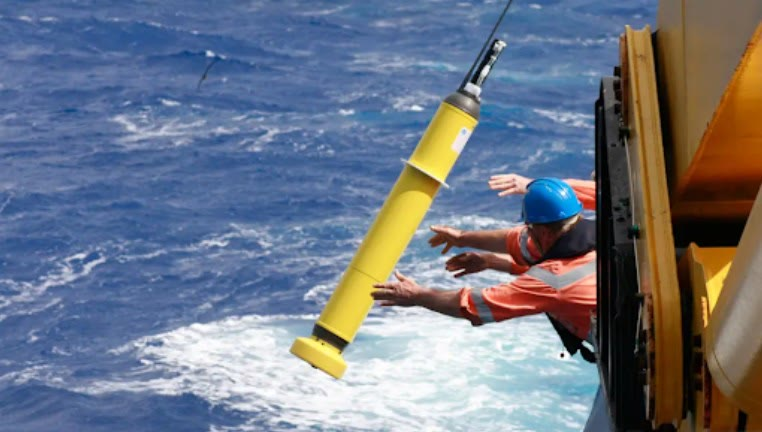
\includegraphics[width=\linewidth]{images/book5/b3-argo-deploy.jpg}

{\scriptsize Um flutuador Argo lançado pela lateral de um navio de pesquisa (NOAA
Global Ocean Monitoring and Observing Program, domínio público).}
\end{minipage}
\end{inthefield}
% ledger: argo:fleet, noaa:argo-25, photo:b3-argo-deploy

\section{Marés oceânicas}\label{sec:b3:ocean-dynamics:tides}

Duas vezes por dia, um pouco menos de uma hora mais tarde a cada dia, o mar sobe e
desce. Os livros de física explicam a força de maré: a atração da Lua é mais intensa
no lado da Terra voltado para a Lua do que no centro, e mais fraca no lado oposto,
de modo que, em relação ao centro, a água é puxada para fora ao longo da linha em direção à Lua,
dos dois lados.

\begin{definition}[Maré de equilíbrio; constituinte de maré]\label{def:b3:ocean-dynamics:tides}
A \emph{maré de equilíbrio}\index{maré de equilíbrio} é a forma que a superfície de um oceano
que cobrisse toda a Terra assumiria se seguisse o potencial gerador de maré
instantaneamente, sem inércia. Um \emph{constituinte de maré}\index{constituinte de maré}
é um dos termos harmônicos, cada um
com uma frequência fixa determinada pelos movimentos da Lua e do Sol e uma
amplitude e fase encontradas em cada lugar, cuja soma produz a maré; são
nomeados por uma letra e pelo número de ciclos por dia, como M$_2$, o
principal constituinte lunar semidiurno.
\end{definition}

\begin{theorem}[Maré de equilíbrio da Lua]\label{thm:b3:ocean-dynamics:equilibrium-tide}
Para a Lua, de massa $M$ a uma distância $d$ do centro da Terra, de
massa $M_E$ e raio $a$, a \omterm{def:b3:ocean-dynamics:tides}{maré de equilíbrio} a um ângulo $\theta$ do
ponto sob a Lua é
\[
\eta = K\,\frac{3\cos^2\theta - 1}{2},\qquad
K = \frac{M}{M_E}\Big(\frac{a}{d}\Big)^3 a .
\]
\end{theorem}

\begin{proof}
O potencial da Lua em um ponto à distância $a$ do
centro da Terra e ângulo $\theta$ é $-GM/s$, com $s^2 = d^2 - 2ad\cos\theta +
a^2$. Expandindo em $a/d$, $1/s = (1/d)[1 + (a/d)\cos\theta + (a/d)^2
(3\cos^2\theta - 1)/2 + \cdots]$. O primeiro termo é uma constante; o segundo
é um campo uniforme, aquele que acelera toda a Terra em sua órbita em torno do
centro de massa comum, e não tem efeito em relação à Terra.
O que resta é o potencial gerador de maré $\Phi_T = -(GMa^2/d^3)(3
\cos^2\theta - 1)/2$. Em equilíbrio, a superfície do mar é uma superfície de
potencial total constante, $g\eta + \Phi_T = C$, com $g = GM_E/a^2$, de modo que
$\eta = (M/M_E)(a^4/d^3)(3\cos^2\theta - 1)/2 + C/g$. A média de
$3\cos^2\theta - 1$ sobre a esfera é zero; como o volume de água é fixo,
$C = 0$.
\end{proof}

Com a razão de massas $0.0123$, $d = \qty{384400}{km}$ e $a =
\qty{6371}{km}$, $K = \qty{0.357}{m}$: o mar fica \qty{0.36}{m}
mais alto sob a Lua e no lado oposto, e \qty{0.18}{m} mais baixo no
grande círculo entre eles, uma amplitude total de \qty{0.54}{m}. Na latitude $\varphi$, com
a Lua na declinação $\delta$ e no ângulo horário $H$, $\cos\theta =
\sin\varphi\sin\delta + \cos\varphi\cos\delta\cos H$. À medida que a Terra gira
sob as duas saliências, um lugar passa por duas preamares em um dia lunar,
\qty{24}{h} \qty{50}{min}: a maré semidiurna. Quando a Lua está
ao norte ou ao sul do equador, as duas saliências ficam inclinadas, e as duas preamares
de um dia são desiguais, como mostra a figura abaixo. O Sol produz uma
maré de mesma forma, com amplitude de \num{0.46} vez a da Lua; as duas se somam na lua nova e
na lua cheia, nas marés de sizígia, e se anulam em parte nas quadraturas.
% ledger: moon5:orbit, earth:Rmean, stewart:tide-equilibrium (computed in figdata/bachelor-3/tides.py)

\begin{omfigure}
\begin{tikzpicture}
\begin{groupplot}[group style={group size=2 by 1, horizontal sep=1.9cm},
  tick label style={font=\scriptsize}, label style={font=\small},
  legend style={font=\scriptsize, draw=none, fill=none}]
\nextgroupplot[width=0.40\linewidth, height=0.40\linewidth, axis equal image, hide axis,
  clip=false, xmin=-1.3, xmax=2.0, ymin=-1.25, ymax=1.25]
% computed in figdata/bachelor-3/tides.py
\addplot[fill=omThm!12, draw=omThm, thick] table[x=x, y=y] {figdata/out/bachelor-3-tides-bulge.dat};
\addplot[black, fill=black!10, domain=0:360, samples=91] ({cos(x)}, {sin(x)});
\draw[->, >=stealth, thick] (axis cs:1.25,0) -- (axis cs:1.95,0);
\node[above, font=\scriptsize, align=center] at (axis cs:1.6,0.08) {para a\\Lua};
\node[font=\scriptsize] at (axis cs:0,0) {Terra};
\nextgroupplot[width=0.54\linewidth, height=0.40\linewidth, xlabel={tempo (\unit{h})},
  ylabel={$\eta$ (\unit{m})}, xmin=0, xmax=49.6, xtick={0,12,24,36,48}, ymin=-0.2, ymax=0.4,
  legend style={at={(axis cs:12.4,0.39)}, anchor=north}, legend cell align=left, legend columns=2]
\addplot[omDef, thick] table[x=t, y=eta0] {figdata/out/bachelor-3-tides-series.dat};
\addlegendentry{$\delta = 0$}
\addplot[omThm, thick] table[x=t, y=eta20] {figdata/out/bachelor-3-tides-series.dat};
\addlegendentry{$\delta = \ang{20}$}
\addplot[black!50, thin, forget plot] coordinates {(0,0) (49.6,0)};
\end{groupplot}
\end{tikzpicture}

\par\smallskip{\small À esquerda, a \omterm{def:b3:ocean-dynamics:tides}{maré de equilíbrio} da Lua, no plano
que contém a Lua, com a saliência exagerada cerca de dois milhões de vezes.
À direita, a \omterm{def:b3:ocean-dynamics:tides}{maré de equilíbrio} em \ang{45} N ao longo de dois dias lunares, com a
Lua no equador (azul) e na declinação \ang{20} N (vermelho): o segundo
caso tem uma preamar bem mais alta que a outra, a
desigualdade diurna.}\label{fig:b3:ocean-dynamics:equilibrium-tide}
\end{omfigure}
% ledger: moon5:orbit, stewart:tide-constituents

A análise harmônica da \omterm{def:b3:ocean-dynamics:tides}{maré de equilíbrio} fornece seus constituintes. As
cinco maiores, com suas amplitudes de equilíbrio, estão na tabela abaixo. Pelo
menos 39 constituintes são necessários para prever a maré de um porto com precisão de um milésimo de
seu maior termo, e um marégrafo deve operar por mais de 18.6 anos, o período
de modulação das marés lunares, para separá-los todos.

\begin{center}
\small
\begin{tabular}{llrr}
\hline
constituinte & origem & período (\unit{h}) & amplitude de equilíbrio (\unit{m}) \\
\hline
M$_2$ & principal lunar, semidiurna & \num{12.4206} & \num{0.2423} \\
S$_2$ & principal solar, semidiurna & \num{12.0000} & \num{0.1128} \\
N$_2$ & lunar elíptica, semidiurna & \num{12.6584} & \num{0.0464} \\
K$_1$ & lunissolar, diurna & \num{23.9344} & \num{0.1416} \\
O$_1$ & principal lunar, diurna & \num{25.8194} & \num{0.1005} \\
\hline
\end{tabular}
\end{center}
% ledger: stewart:tide-constituents, stewart:tide-prediction

A maré real não é a \omterm{def:b3:ocean-dynamics:tides}{maré de equilíbrio}. Para manter uma saliência sob a Lua
no equador, a maré teria de percorrer a Terra em um dia lunar,
a cerca de \qty{460}{m/s}, velocidade que uma onda longa de gravidade atinge apenas
em um oceano de \qty{22}{km} de profundidade; e os continentes a detêm. A maré é
antes uma onda longa forçada, oscilando em cada bacia perto da ressonância, e a
rotação da Terra faz com que ela circule em torno da bacia.
% ledger: stewart:tide-prediction

\begin{definition}[Onda de Kelvin]\label{def:b3:ocean-dynamics:kelvin-wave}
Uma \emph{onda de Kelvin}\index{onda de Kelvin} oceânica é uma onda longa de gravidade
que se propaga ao longo de uma costa, ou ao longo do equador, sem velocidade
transversal a ela, com sua altura decaindo exponencialmente à medida que se afasta da costa, a
distância da ordem do raio de Rossby. Ao longo de uma costa, ela se propaga com a costa à
sua direita no Hemisfério Norte, e à sua esquerda no Hemisfério Sul.
\end{definition}

\begin{theorem}[Onda de Kelvin costeira]\label{thm:b3:ocean-dynamics:kelvin}
Em um oceano de profundidade uniforme $H$ sobre um plano $f$, com $f > 0$, limitado por uma
costa retilínea ao longo de $y = 0$, situado em $y > 0$, as equações lineares de águas rasas
têm soluções com $v = 0$
\[
\eta = \mathrm e^{-y/L_R}F(x - ct),\qquad u = \frac{g}{c}\,\eta,\qquad
c = \sqrt{gH},\quad L_R = \frac{c}{f},
\]
para qualquer perfil $F$, e nenhuma solução com $v = 0$ se propaga no sentido
$-x$.
\end{theorem}

\begin{proof}
Com $v = 0$, as equações são $\partial u/\partial t = -g\,\partial\eta/
\partial x$, $fu = -g\,\partial\eta/\partial y$ e $\partial\eta/\partial t
+ H\,\partial u/\partial x = 0$. A primeira e a terceira fornecem $\partial^2
\eta/\partial t^2 = gH\,\partial^2\eta/\partial x^2$: em $x$, cada linha
$y = $ const transporta ondas $F(x \mp ct)$ com $c = \sqrt{gH}$, e então a
primeira equação fornece $u = \pm(g/c)\eta$. A segunda fica $\partial\eta/
\partial y = \mp(f/c)\eta$, logo $\eta \propto \mathrm e^{\mp y/L_R}$. Com
o sinal superior, a onda decai afastando-se da costa; com o inferior, ela
cresceria sem limite para dentro do oceano, o que é excluído. A onda se propaga
no sentido de $+x$, com o oceano à sua esquerda e a costa à direita.
\end{proof}

Sobre o oceano profundo, com \qty{4000}{m} de profundidade, $c = \qty{198}{m/s}$ e o
raio de Rossby é de cerca de \qty{2000}{km} em latitudes médias: a maré percorre
toda a bacia. Sobre um mar de plataforma com \qty{50}{m} de profundidade, $c =
\qty{22}{m/s}$, o raio de Rossby é menor que \qty{200}{km}, e um comprimento de onda de M$_2$
é de cerca de \qty{1000}{km}. Em um golfo, a maré que entra por uma
costa como \omterm{def:b3:ocean-dynamics:kelvin-wave}{onda de Kelvin} retorna pela costa oposta, de novo com a
costa à direita; as duas ondas se anulam em pontos intermediários.

\begin{definition}[Ponto anfidrômico; linha cotidal; linha de igual amplitude]\label{def:b3:ocean-dynamics:amphidrome}
Um \emph{ponto anfidrômico}\index{ponto anfidrômico} é um ponto em que a
amplitude de uma \omterm{def:b3:ocean-dynamics:tides}{constituinte de maré} é nula e em torno do qual sua preamar
gira. Uma \emph{linha cotidal}\index{linha cotidal} une os lugares em que a
preamar de uma constituinte ocorre no mesmo instante; uma \emph{linha de
igual amplitude}\index{linha de igual amplitude} une os lugares de mesma amplitude de maré. As linhas cotidais
irradiam-se dos pontos anfidrômicos; as linhas de igual amplitude os circundam.
\end{definition}

\begin{omfigure}
\centering
\begin{tikzpicture}
\begin{axis}[width=0.96\linewidth, height=0.35\linewidth, axis equal image,
  xmin=0, xmax=1600, ymin=0, ymax=400, xtick={0,400,800,1200,1600}, ytick={0,200,400},
  xlabel={distância ao longo do canal (\unit{km})}, ylabel={transversal (\unit{km})},
  tick label style={font=\scriptsize}, label style={font=\small}]
% computed in figdata/bachelor-3/tides.py
\addplot[omDef!70, densely dashed, unbounded coords=jump] table[x=x, y=y] {figdata/out/bachelor-3-tides-cor.dat};
\pgfplotsinvokeforeach{30,60,90,120,150,180,210,240,270,300,330}{
  \addplot[omThm, thin, unbounded coords=jump] table[x=x, y=y] {figdata/out/bachelor-3-tides-cot-#1.dat};
}
\addplot[omThm, very thick, unbounded coords=jump] table[x=x, y=y] {figdata/out/bachelor-3-tides-cot-0.dat};
\addplot[only marks, mark=*, mark size=2pt] table[x=x, y=y] {figdata/out/bachelor-3-tides-amph.dat};
\addplot[->, >=stealth, very thick, domain=20:310, samples=60] ({742.7+70*cos(x)}, {200+70*sin(x)});
\end{axis}
\end{tikzpicture}

\par\smallskip{\small Duas \omterm{def:b3:ocean-dynamics:kelvin-wave}{ondas de Kelvin} da maré M$_2$ em um canal fictício
com \qty{400}{km} de largura e \qty{50}{m} de profundidade a \ang{55} N, uma indo
para L ao longo da costa sul, a outra para O ao longo da costa norte.
Em vermelho, as linhas cotidais, a cada \ang{30} de fase (cerca de uma hora), a
mais grossa para a preamar na origem do tempo; em azul tracejado, as \omterm{def:b3:ocean-dynamics:amphidrome}{linhas de
igual amplitude}, em intervalos de um quinto da amplitude de uma onda em sua costa. Os
\omterm{def:b3:ocean-dynamics:amphidrome}{pontos anfidrômicos} (bolinhas) situam-se sobre a linha central, separados por meio comprimento de onda,
\qty{495}{km} entre si, e a preamar gira em torno deles no sentido anti-horário
(seta).}\label{fig:b3:ocean-dynamics:amphidromes}
\end{omfigure}

Os mapas da maré oceânica feitos a partir de altimetria por satélite, com precisão de cerca de
\qty{2}{cm} em mar profundo, mostram essa estrutura em toda parte: a crista de M$_2$
gira no sentido anti-horário em torno dos \omterm{def:b3:ocean-dynamics:amphidrome}{pontos anfidrômicos} das bacias do Hemisfério Norte
e no sentido horário no Hemisfério Sul, e as maiores amplitudes estão nas
costas. As marés dissipam \qty{3.75}{TW}, \qty{3.5}{TW} dos quais no
oceano, cerca de dois terços da energia de M$_2$ nas plataformas e nos mares rasos e
um terço por ondas internas no oceano profundo. Essa energia
alonga o dia em cerca de \qty{2.07}{ms} por século e afasta a Lua
em \qty{3.86}{cm} por ano; e a parte dissipada no oceano profundo mistura essas águas,
fornecendo parte da mistura que, no quadro de Stommel--Arons, impulsiona
a circulação abissal.
% ledger: stewart:tide-prediction


\section{Exercícios}

\begin{exercise}[$\star$]\label{exo:b3:ocean-dynamics:1}
Uma tensão do vento de oeste de \qty{0.12}{Pa} sopra sobre o mar a \ang{40} N
($\rho = \qty{1025}{kg/m^3}$, $\Omega = \qty{7.292115e-5}{rad/s}$).
Calcule o transporte volumétrico de Ekman por metro de largura e sua direção,
e o transporte através de uma seção de \qty{1000}{km} de comprimento, em sverdrups.
\end{exercise}

\begin{exercise}[$\star$]\label{exo:b3:ocean-dynamics:2}
Com $A_z = \qty{0.05}{m^2/s}$, calcule a \omterm{def:b3:ocean-dynamics:ekman-pumping}{profundidade de Ekman} a \ang{45} N. Qual
fração da corrente superficial permanece nessa profundidade?
\end{exercise}

\begin{exercise}[$\star$]\label{exo:b3:ocean-dynamics:3}
A \ang{30} N, o rotacional da tensão do vento é \qty{-1e-7}{Pa/m} em uma
bacia de \qty{5000}{km} de largura ($a = \qty{6371}{km}$). Calcule $\beta$, o
transporte de Sverdrup por unidade de largura e o transporte total, com sua
direção.
\end{exercise}

\begin{exercise}[$\star$]\label{exo:b3:ocean-dynamics:4}
A partir dos períodos de M$_2$ e S$_2$, calcule o período do ciclo de
marés de sizígia e de quadratura, o intervalo de tempo entre dois alinhamentos das duas
constituintes.
\end{exercise}

\begin{exercise}[$\star\star$]\label{exo:b3:ocean-dynamics:5}
Uma tensão do vento de oeste cresce linearmente de 0 em \ang{35} N até \qty{0.1}{Pa} em
\ang{45} N, a \qty{1110}{km} mais ao norte. Calcule o \omterm{def:b3:ocean-dynamics:ekman-pumping}{bombeamento de Ekman} em
\ang{40} N, mantendo os dois termos da \cref{prop:b3:ocean-dynamics:pumping}, em
metros por ano. A água é empurrada para cima ou para baixo?
\end{exercise}

\begin{exercise}[$\star\star$]\label{exo:b3:ocean-dynamics:6}
Em um giro de Stommel com $r = \qty{2e-6}{s^{-1}}$ e $\beta =
\qty{2e-11}{m^{-1}.s^{-1}}$, calcule a largura $\delta_S$. Se a
corrente de contorno transporta \qty{30}{\sverdrup} nos \qty{800}{m} superiores, dentro de uma
largura $\delta_S$, qual é a sua velocidade média?
\end{exercise}

\begin{exercise}[$\star\star$]\label{exo:b3:ocean-dynamics:7}
Calcule a largura de Munk $\delta_M$ e a largura do jato para o norte,
$(2\pi/\sqrt3)\,\delta_M$, em \ang{30} N para $A_H = \qty{e4}{m^2/s}$. Como
a largura muda se $A_H$ for oito vezes menor?
\end{exercise}

\begin{exercise}[$\star\star$]\label{exo:b3:ocean-dynamics:8}
Duas estações distantes \qty{80}{km} entre si estão sobre uma linha que vai de oeste ($A$)
a leste ($B$), em \ang{36} N. Em relação à superfície de \qty{1000}{dbar}, a
anomalia \omterm{def:b3:gravity-geodesy:geopotential}{geopotencial} da superfície do mar é \qty{14.5}{J/kg} em $A$ e
\qty{21.3}{J/kg} em $B$. Calcule a corrente superficial em relação a
\qty{1000}{dbar} e sua direção. Qual estação tem a coluna de água
mais quente?
\end{exercise}

\begin{exercise}[$\star\star$]\label{exo:b3:ocean-dynamics:9}
Com a \omterm{def:b3:ocean-dynamics:tides}{maré de equilíbrio} da Lua, $K = \qty{0.357}{m}$, e a razão
\num{0.46} da maré solar para a lunar, calcule a amplitude de equilíbrio
(preamar sob os astros menos baixa-mar a \ang{90}) em marés de sizígia e
de quadratura, e a razão entre elas.
\end{exercise}

\begin{exercise}[$\star\star\star$]\label{exo:b3:ocean-dynamics:10}
No plano $\beta$ equatorial, $f = \beta_0y$ com $\beta_0 =
2\Omega/a$. Mostre que a \omterm{def:b3:ocean-dynamics:kelvin-wave}{onda de Kelvin} $\eta = G(y)F(x - ct)$, $v = 0$,
torna-se $G = \exp(-\beta_0y^2/2c)$, aprisionada em ambos os lados do equador,
e propaga-se para leste. Calcule sua escala de aprisionamento $\sqrt{c/\beta_0}$ para uma
onda de velocidade \qty{2.5}{m/s}.
\end{exercise}

\begin{exercise}[$\star\star\star$]\label{exo:b3:ocean-dynamics:11}
(a)~Deduza $V = a\tan\varphi\,W_0$ para o interior abissal a partir de $\beta v =
f\,\partial w/\partial z$. (b)~Com $W_0 = \qty{e-7}{m/s}$, calcule $V$ em
\ang{30} N e o transporte total em direção ao polo através de uma bacia
de \qty{5000}{km} de largura. (c)~De onde deve vir a água?
\end{exercise}

\begin{exercise}[$\star\star\star$]\label{exo:b3:ocean-dynamics:12}
Uma corrente geostrófica $W_g = u_g + \mathrm iv_g$ escoa sobre um fundo marinho plano
em $z = 0$, com viscosidade de turbilhão $A_z$ e sem deslizamento no fundo.
(a)~Mostre que $W = W_g(1 - \mathrm e^{-(1+\mathrm i)z/\delta})$, $\delta =
\sqrt{2A_z/f}$. (b)~Mostre que o déficit de transporte desta camada de Ekman
de fundo bombeia a velocidade vertical $w = \tfrac12\delta\zeta_g$ para o
interior, sendo $\zeta_g$ a vorticidade da corrente geostrófica. (c)~Para
$A_z = \qty{0.01}{m^2/s}$, $f = \qty{e-4}{s^{-1}}$ e um oceano
de \qty{4000}{m} de profundidade, calcule $\delta$, a taxa de desaceleração $r =
f\delta/2H$, e seu inverso, em dias.
\end{exercise}
% ledger: earth:Rmean, geod5:grs80-defining, stewart:tide-constituents, stewart:tide-equilibrium

\section{Problema: Um giro no mar de Ammar}

\begin{problem}[{Problema de fim de semana --- bombeamento de Ekman, transporte de Sverdrup,
a corrente de contorno oeste e a maré de um oceano inventado}]
\label{pb:b3:ocean-dynamics:1}
O mar de Ammar é uma bacia oceânica inventada, um retângulo de \ang{20} a
\ang{50} N e \qty{6000}{km} de largura, \qty{4000}{m} de profundidade. A tensão do vento é
zonal, $\tau_x = -\tau_0\cos(\pi(\varphi - \ang{20})/\ang{30})$ com $\tau_0
= \qty{0.1}{Pa}$. Considere $\rho = \qty{1025}{kg/m^3}$, $\Omega =
\qty{7.292115e-5}{rad/s}$, $a = \qty{6371}{km}$, $g = \qty{9.81}{m/s^2}$,
e, quando se pedir um plano $\beta$, seu valor em \ang{35} N.

\medskip\noindent\textbf{Parte I --- A camada de Ekman.}
\begin{enumerate}
\item Calcule a tensão do vento em \ang{20}, \ang{35} e \ang{50} N.
\item Calcule $f$ nas mesmas latitudes.
\item Calcule o transporte de volume de Ekman por unidade de largura em \ang{20} e
  \ang{50} N, com sua direção. Os transportes convergem ou divergem na
  bacia?
\item Com $A_z = \qty{0.05}{m^2/s}$, calcule a \omterm{def:b3:ocean-dynamics:ekman-pumping}{profundidade de Ekman} em \ang{35} N.
\item Calcule o \omterm{def:b3:ocean-dynamics:ekman-pumping}{bombeamento de Ekman} em \ang{35} N, em metros por segundo e por
  ano.
\item Quantos anos levaria este bombeamento para empurrar a água superficial
  para baixo \qty{500}{m}?
\end{enumerate}

\medskip\noindent\textbf{Parte II --- O interior de Sverdrup.}
\begin{enumerate}[resume]
\item Calcule o comprimento $L$ da bacia do sul ao norte e $\beta$ em
  \ang{35} N.
\item Calcule o rotacional da tensão do vento em \ang{35} N.
\item Calcule o transporte de Sverdrup por unidade de largura em \ang{35} N, com sua
  direção.
\item Calcule o transporte interior total através da bacia em \ang{35} N,
  em sverdrups.
\item Se este escoamento estiver distribuído nos primeiros \qty{1000}{m}, qual é sua
  velocidade média, e quantos anos uma parcela leva para se deslocar \qty{1000}{km}
  para o sul?
\item Mostre que $fw_E/\beta$ em \ang{35} N fornece o mesmo transporte, e
  explique o porquê com a \omterm{def:b3:atmospheric-dynamics:pv}{vorticidade potencial} de uma coluna.
\end{enumerate}

\medskip\noindent\textbf{Parte III --- A corrente de contorno oeste.}
\begin{enumerate}[resume]
\item Explique por que o escoamento de retorno não pode correr ao longo do lado leste da
  bacia.
\item Com um atrito de fundo $r = \qty{e-6}{s^{-1}}$, calcule a
  largura de Stommel $\delta_S$.
\item Calcule o transporte para o norte por unidade de largura na parede oeste,
  $A(X/\delta_S - 1)$, e a velocidade média se ela preencher a
  camada superior de \qty{1000}{m}.
\item A que distância da parede termina o escoamento para o norte?
\item Calcule o transporte para o norte da camada limite de Stommel, e
  explique por que ele fica aquém do transporte interior em cerca de
  \qty{1.5}{\sverdrup}.
\item Com $A_H = \qty{5e3}{m^2/s}$, calcule $\delta_M$ e a largura do
  jato para o norte de Munk.
\item O jato de Munk transporta $1 + \mathrm e^{-\pi/\sqrt3}$ vezes o
  transporte interior. Calcule-o e diga para onde vai o excesso.
\end{enumerate}

\medskip\noindent\textbf{Parte IV --- A maré do mar de Ammar.}
\begin{enumerate}[resume]
\item Calcule a velocidade de uma \omterm{def:b3:ocean-dynamics:kelvin-wave}{onda de Kelvin} na bacia e o raio de Rossby
  em \ang{35} N.
\item Calcule o comprimento de onda da \omterm{def:b3:ocean-dynamics:kelvin-wave}{onda de Kelvin} associada a M$_2$.
\item Quanto tempo uma \omterm{def:b3:ocean-dynamics:kelvin-wave}{onda de Kelvin} leva para dar uma volta completa ao longo das costas da
  bacia, e quantos períodos de M$_2$ isso representa?
\item Com que velocidade a \omterm{def:b3:ocean-dynamics:tides}{maré de equilíbrio} precisaria percorrer o
  círculo de \ang{35} N para permanecer sob a Lua, e em que profundidade de oceano
  uma onda longa se propagaria com essa velocidade?
\item Indique onde deve estar o \omterm{def:b3:ocean-dynamics:amphidrome}{ponto anfidrômico} da bacia, e em que
  sentido a preamar gira ao redor dele?
\item Calcule a amplitude de equilíbrio semidiurna em \ang{35} N, $\tfrac34
  K\cos^2\varphi$, com $K = \qty{0.357}{m}$, para a Lua sobre o equador.
\item Dê o transporte da corrente de contorno oeste que fecha o
  giro do mar de Ammar.
\end{enumerate}
\end{problem}
% ledger: earth:Rmean, geod5:grs80-defining, stewart:tide-constituents
